\title{Fit Function}
\author{Jinfu Leng}
\documentclass[12pt]{article}
\usepackage{graphicx}
\begin{document}
\maketitle

\section{Intorduction}
The camera was set to the origin of the coordinate system. The ball was throwed toward the camera from the front. (We suppose that the ball is in the center in the horizontal direction all the time)

Theoretically, the function should be:
\begin{itemize}
\item $x - 3 = -3 * t$ (the initial position of the ball is x = 3, and the initial xlinear speed is -3)
\item $y + 0.44 = 4 * t - 1/2 * 10 * t^{2}$ (the initial position of the ball is y=-0.44, and the initial ylinear speed is 4)
\end{itemize}
Based on the two equations above, we can get the theoretical function:
$y = -5/9 * x^{2} + 2x - 1.44$
\section{Chart}
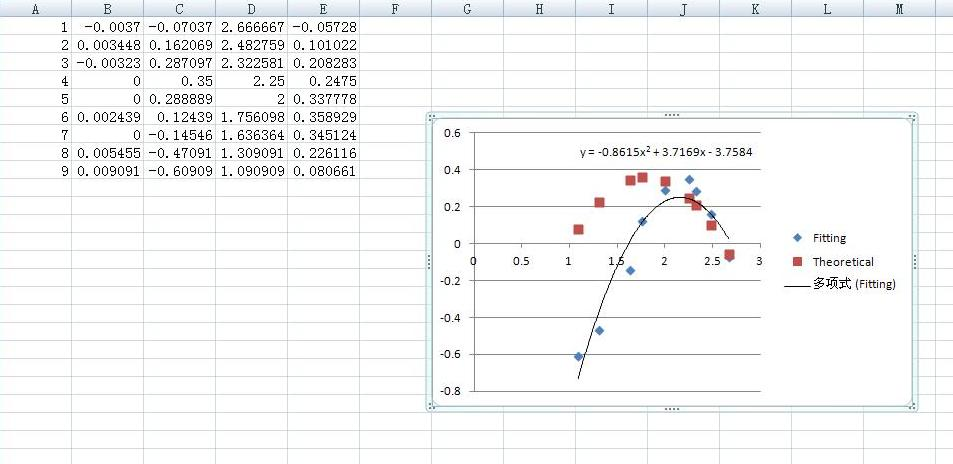
\includegraphics[scale = 0.5]{../../fit_function.jpg}
\begin{itemize}
\item The blue points: the experiment result
\item The black line: fitted function based on the experiment result
\item The red points: the theoretical result
\end{itemize}
\section{Explanations}
The experiment result showed a parabola curve. Especially, when the ball is relatively far away from the ball, the theoretical result and the experiment result matched quite well. But the difference increased when the ball is relatively close to the camera. Based on my observation, the errors may come from the overestimation of the distance, especially when the ball is close.
\section{Next?}
Firstly, I want to check if the ball really worked like the theoretical function. Then, I will do more experiments to see if other throwing has similar results as the above chart showed. If yes, I think we need to improve the accuracy level of positioning the ball. For example, consier the curvature of the ball, compute the x-radius and y-radius of the ball seperately.
\end{document}